\documentclass[12pt]{article}
\usepackage[pdfborder={0 0 0.5 [3 2]}]{hyperref}%
\usepackage[left=1in,right=1in,top=1in,bottom=1in]{geometry}%
\usepackage[shortalphabetic]{amsrefs}%
\usepackage{amsmath}
\usepackage{enumerate}
\usepackage{enumitem}
\usepackage{amssymb}                
\usepackage{amsmath}                
\usepackage{amsfonts}
\usepackage{amsthm}
\usepackage{bbm}
\usepackage[table,xcdraw]{xcolor}
\usepackage{tikz}
\usepackage{float}
\usepackage{booktabs}
\usepackage{svg}
\usepackage{mathtools}
\usepackage{cool}
\usepackage{url}
\usepackage{graphicx,epsfig}
\usepackage{framed}
\usepackage{hyperref}  

\usetikzlibrary{automata,arrows,positioning,calc}
\DeclarePairedDelimiter\abs{\lvert}{\rvert}%
\DeclarePairedDelimiter\norm{\lVert}{\rVert}%
\DeclarePairedDelimiter\ceil{\lceil}{\rceil}
\DeclarePairedDelimiter\floor{\lfloor}{\rfloor}

\makeatletter
\renewcommand*\env@matrix[1][*\c@MaxMatrixCols c]{%
  \hskip -\arraycolsep
  \let\@ifnextchar\new@ifnextchar
  \array{#1}}
\makeatother

\newtheorem{theorem}{Theorem}[section]
\newtheorem{corollary}{Corollary}[theorem]
\newtheorem{proposition}[theorem]{Proposition}
\newtheorem{lemma}[theorem]{Lemma}

\theoremstyle{definition}
\newtheorem{definition}[theorem]{Definition}
\newtheorem{exercise}{Exercise}%
\newtheorem{problem}[exercise]{Problem}%
\newtheorem*{example}{Example}

\theoremstyle{remark}
\newtheorem*{question}{Question}
\newtheorem*{observation}{Observation}
\newtheorem*{remark}{Remark}

\graphicspath{ {images/} }

\setlength{\parindent}{0cm}
\renewcommand{\vec}[1]{\ensuremath{\mathbf{#1}}}

\def\noi{\noindent}
\def\T{{\mathbb T}}
\def\R{{\mathbb R}}
\def\N{{\mathbb N}}
\def\C{{\mathbb C}}
\def\Z{{\mathbb Z}}
\def\P{{\mathbb P}}
\def\E{{\mathbb E}}
\def\Q{\mathbb{Q}}
\def\ind{{\mathbb I}}

\def\cale{{\mathcal E}}
\def\cals{{\mathcal S}}
\def\calc{{\mathcal C}}
\def\caln{{\mathcal N}}
\def\calb{{\mathcal B}}
\def\calg{{\cal G}}

\def\ds{\displaystyle}
\def\ra{\rightarrow}
\newcommand{\conv}{\mbox{\rm conv}}
\newcommand{\spaan}{\mbox{\rm span}}
\newcommand{\deet}{\mbox{\rm det}}
\newcommand{\aff}{\mbox{\rm aff}}
\newcommand{\cl}{\mbox{\rm cl}}
\newcommand{\dimm}{\mbox{\rm dim}}
\newcommand{\sm}{\setminus}
\def\ci{\perp\!\!\!\perp}

\newcommand{\ink}{\rule{.5\baselineskip}{.55\baselineskip}}

\begin{document}

\setcounter{section}{2}
\section{Continuous Random Variables}

\subsection{Introduction}
Many quantities of interest in the real world are not discrete is nature. Examples include the following:
\begin{enumerate}
\item The amount of rainfall in one day
\item The weight of an adult chimpanzee
\item The functional lifetime of an O-ring in a jet engine
\end{enumerate}

A random variable which can take on any value within a range is called a \emph{continuous random variable}. These are fundamentally different from discrete random variables in the following way. Recall that to specify a discrete random variable, all we have to do is assign probabilities between 0 and 1 to every possible output of the random variable in such a way that all the probabilities add up to 1. This is not possible for a random variable which can take values in an interval on the real number line. We must, therefore, use a different technique to describe a continuous random variable. Here will we use calculus for (essentially) the first time in the course.

\subsection{Probability Density Functions}
For a continuous random variable, rather than talk about the probability that a random variable equals a particular value, we talk about the probability that a random value falls within a particular range. (In fact, as we will see, the probability that a continuous random variable equals a specific value is 0.) A continuous random variable is described by a \emph{probability density function (pdf)}. Here are examples of pdfs:

\begin{figure}[H]
\centering
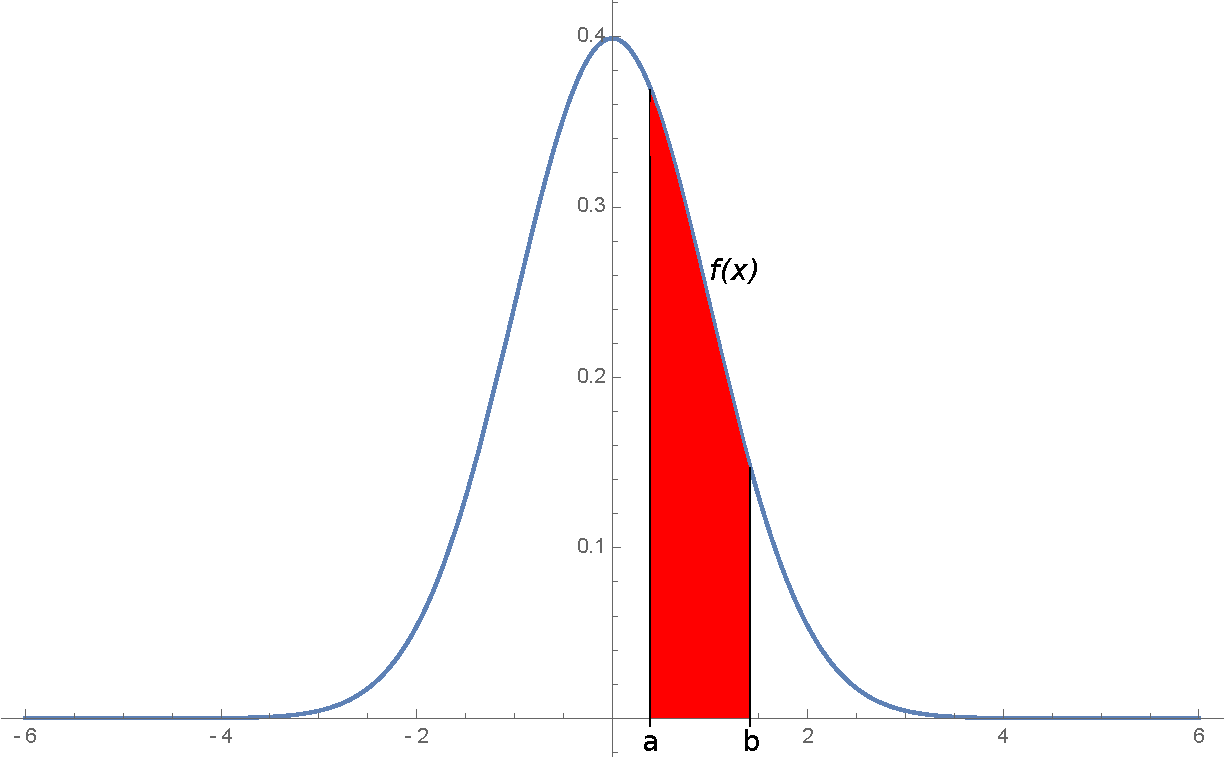
\includegraphics[width=8cm]{normalpdf}
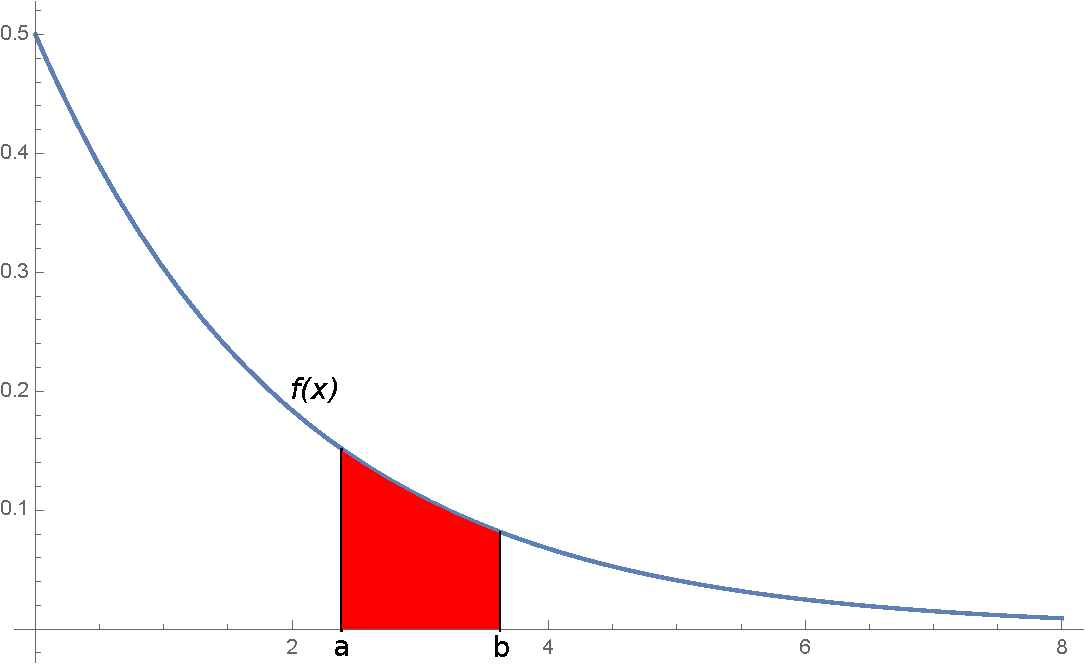
\includegraphics[width=8cm]{exppdf}
\end{figure}

A pdf is a nonnegative function $f(x)$ where the total area under the curve is 1 (this is analagous to the discrete case where the probabilities of all the outputs sum to 1). The probability that a random variable falls into an interval $[a, b]$ is the area under the density curve between $a$ and $b$. This is illustrated in red in the above pdfs. Since we are talking about areas under curves, we need to use calculus. In particular, we need to integrate! Here is the formal definition of a pdf:

\begin{framed}
\emph{Probability Density Function (pdf)}\\
  \rule{\dimexpr\linewidth-2\fboxsep-2\fboxrule}{.1pt} \\
The function $f(y)$ is a \emph{probabiltiy density function} (pdf) for a continuous random variable $Y$ if $f(y) \geq 0$ for all $y$, and
\[
\int_{-\infty}^\infty f(y) dy = 1
\]
The probability that $Y$ falls into the interval $[a, b]$ is the area under the density curve between $a$ and $b$, i.e.
\[
\P(a \leq Y \leq b) = \int_a^b f(y) dy
\]
\end{framed}

Before we continue, let's mention one way in which continuous and discrete distributions are very different. For a continuous distribution, the probability of any single point is 0. We can see that from the density function since for a continuous random variable $Y$ with density $y$,
\[
\P(Y = a) = \int_a^a f(y) dy = 0
\]
Thus all the following probabilities are the same:
\[
\P(a \leq Y \leq b) = \P(a \leq Y < b) = \P(a < Y \leq b) = \P(a < Y < b) = \int_a^b f(y) dy
\]
In other words, it does not matter which inequality sign (< or $\leq$) we use for the endpoints of the interval since the probability of hitting the endpoints in 0. This is not at all the case for the discrete case, where individual points have positive probability. If $X$ is the number of flips of heads in 20 tosses of a fair coin, then $\P(8 \leq X \leq 12)$ and $\P(8 < X \leq 12)$ are very different!

\begin{example}Consider the function
\[
f(y) = \begin{cases}
cy^2 & 0 \leq y\leq 2\\
0 & \text{otherwise}
\end{cases}
\]
\begin{enumerate}
\item Find the value of $c$ for which $f(y)$ is a valid density function.

First note that $f(y)$ is nonnegative, so there is nothing to worry about there. Next we need to make sure that the density function integrates to 1.
\begin{align*}
1 &= \int_{-\infty}^\infty f(y) dy \\
&= \int_0^2 c y^2 dy &\text{since $f(y)$ is 0 outside $[0, 2]$}\\
&= c\frac{y^3}{3}\Bigr|_0^2 \\
&= \frac{8}{3}c
\end{align*}
Thus, choosing $c = 3/8$, we have a valid density function.

\item What is $P(1 \leq Y \leq 2)$?\\

Integrating the density function from 1 to 2, we get:
\begin{align*}
\P(1 \leq Y \leq 2) &= \int_1^2 f(y) dy \\
&= \int_1^2 \frac{3}{8} y^2 dy \\
&= \frac{3}{8} \frac{y^3}{3} \Bigr|_1^2\\
&= \frac{7}{8}
\end{align*}

\end{enumerate}
\end{example}

\subsection{Cumulative Distribution Functions}
Another way to describe a continuous random variable is with its \emph{cumulative distribution function} (cdf)\footnote{Sometimes you will see this called simply a \emph{distribution function}. I will always use the term cdf.}.\\

\begin{framed}
\emph{Cumulative Distribution Function (cdf)}\\
  \rule{\dimexpr\linewidth-2\fboxsep-2\fboxrule}{.1pt} \\
Let $Y$ be a random variable. The the \emph{cumulative distribution function} cdf of $Y$, denoted $F(y)$, is defined by
\[
F(y) = \P(Y \leq y)
\]
If $Y$ has density function $f(y)$, then
\[
F(y) = \int_{-\infty}^y f(y) dy
\]
\end{framed}

The cdf gives the probability that our random variable $Y$ is less than or equal to a certain value. For a continuous random variable, $F(y)$ can be visualized graphically as the area under the density curve to the left of $y$.

\begin{figure}[H]
\centering
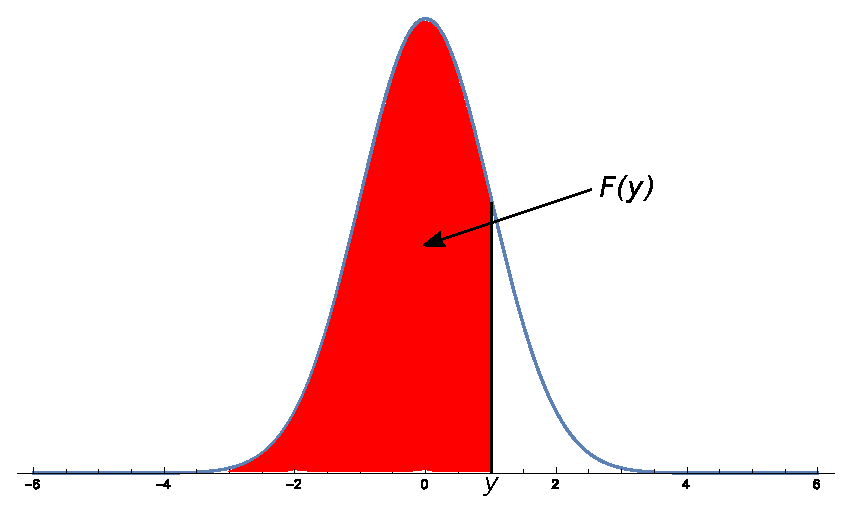
\includegraphics[width=8cm]{normalcdf.eps}
\end{figure}

Note that traditionally the cdf is written with an uppercase $F$, while the density is written with a lowercase $f$.
The cdf is defined for discrete as well as continuous random variables, although we will never use it in the discrete case\footnote{The cdf for a discrete random variable is always a step function, since the cdf only increases on the finite or countable set of points which have positive probabilities.}. The cdf has the following properties.

\begin{framed}
\emph{Properties of cdfs}\\
  \rule{\dimexpr\linewidth-2\fboxsep-2\fboxrule}{.1pt} \\
Let $Y$ be a random variable with cdf $F(y)$. Then:
\begin{enumerate}
\item $F(y)$ is a nondecreasing function.
\item $\lim_{y \rightarrow -\infty} F(y) = 0$
\item $\lim_{y \rightarrow \infty} F(y) = 1$
\item For a continuous random variable $Y$, the cdf $F(y)$ is a continuous function.
\end{enumerate}
\end{framed}

For a continuous random variable, the cdf and pdf are related via the fundamental theorem of calculus. 

\begin{framed}
\emph{Relationship between cdf and pdf}\\
  \rule{\dimexpr\linewidth-2\fboxsep-2\fboxrule}{.1pt} \\
Let $Y$ be a continuous random variable with cdf $F(y)$ and density $f(y)$. Then we have the following relationships:
\begin{enumerate}
\item 
\[
F(y) = \int_{\infty}^y f(y) dy
\]

\item
\[
f(y) = \frac{DF(y)}{dy} = F'(y)
\]
\item
\[
\P(a \leq Y \leq b) = \int_a^b f(y) dy = F(b) - F(a)
\]
\end{enumerate}
\end{framed}

We can illustrate the third relationship above, $\P(a \leq Y \leq b) = F(b) - F(a)$, using the graphs below. You can see that subtracting the first area from the second area yields the third area.
\begin{figure}[H]
\centering
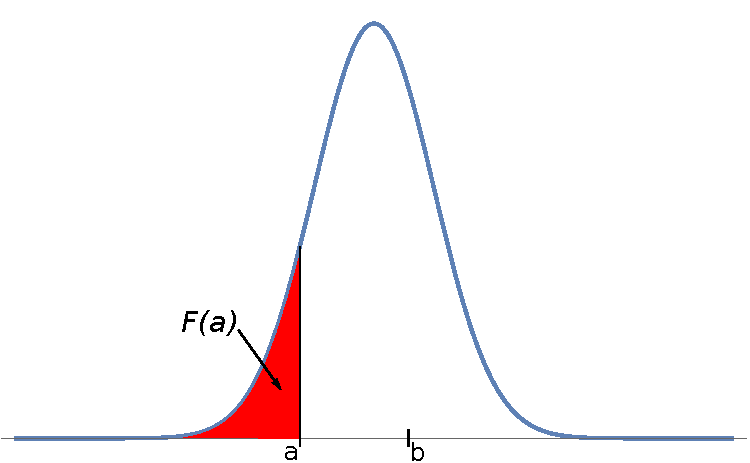
\includegraphics[width=5cm]{normalcdfFa.pdf}
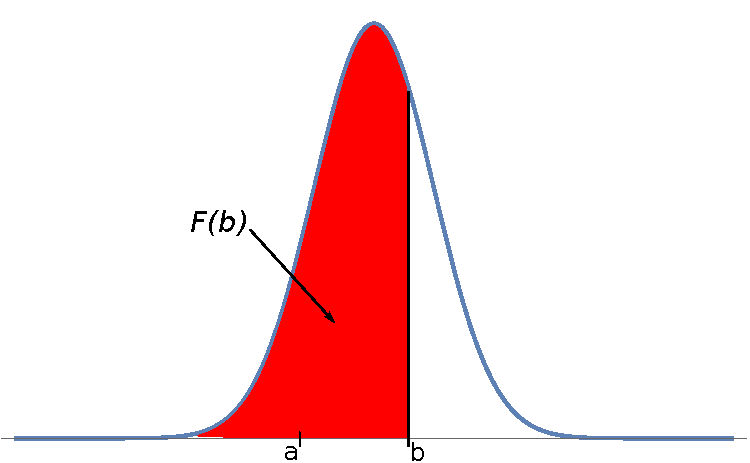
\includegraphics[width=5cm]{normalcdfFb.pdf}
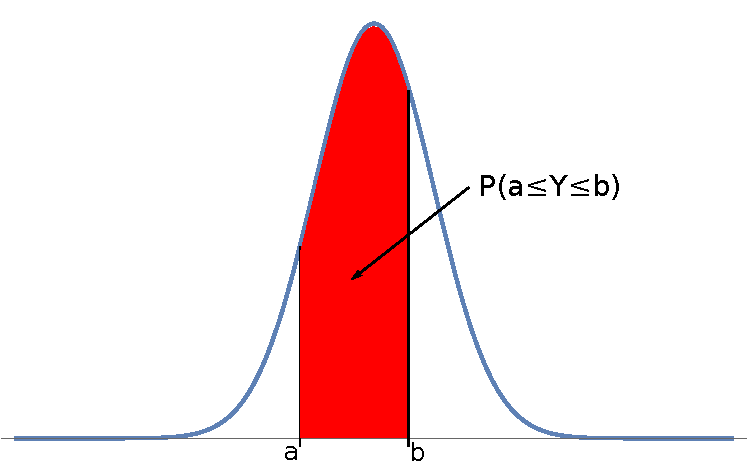
\includegraphics[width=5cm]{normalcdfPab.pdf}
\end{figure}

You may ask why we bother at all with cdfs since it seems easier to work with densities. There are three good reasons to consider CDFs. From a mathematical standpoint, the cdf is a more fundamental object than the pdf; every continuous random variable has a cdf, while there are continuous random variables which have no density\footnote{All continuous random variables we will encounter in this course will have a density}. From a practical standpoint, the normal distribution, perhaps the most important distribution is all of probabiltiy, has a density which is unwieldy, thus we will use the cdf to compute probabilities involving that distribution. Finally, the cdf is used to define the \emph{median} and \emph{quartlies} of a probability distribution, which are important descriptors of a probability distribution.

\subsection{Median and Quartiles}
The \emph{median} is the ``middle'' of a probability distribution. It is the value which separates the upper half of the distribution from the lower half of the distribution. The median is more robust to outlier values than the mean, and so in some cases may be a better descriptor of a typical outcome than the mean. Mathematically, if $Y$ is a random variable, the we can define the median of $Y$ as the value $m$ such that $\P(Y \leq m) = \P(Y \geq m) = 1/2$. For a continuous random variable $Y$ with cdf $F(y)$, we can define the median using the cdf as the value $m$ for which $F(m) = 1/2$. Similarly we can define the 1st and 3rd quartiles (the median is sometimes called the 2nd quartile). 

\begin{framed}
\emph{Median and quartiles}\\
  \rule{\dimexpr\linewidth-2\fboxsep-2\fboxrule}{.1pt} \\
Let $Y$ be a continuous random variable with cdf $F(y)$. Then we define the \emph{median} $m$, \emph{first quartile} $Q_1$, and \emph{third quartile} $Q_3$ by the following relationships:
\begin{align*}
F(Q_1) &= \P(Y \leq Q_1) = 1/4\\
F(m) &= \P(Y \leq m) = 1/2\\
F(Q_3) &= \P(Y \leq Q_3) = 1/4
\end{align*}
\end{framed}

Let's revisit our example from the previous section.

\begin{example}
Let $Y$ be a continuous random variable with density $f(y)$ defined by
\[
f(y) = \begin{cases}
\frac{3}{8} y^2 & 0 \leq y\leq 2\\
0 & \text{otherwise}
\end{cases}
\]
Find the median of $Y$.\\

Let $m$ be the median of $Y$. Since $F(m) = 1/2$, where $F(y)$ is the cdf of $Y$, we need to first find the cdf. For $y < 0$, $F(y) = 0$ and for $y > 2$, $F(y) = 1$ (do you see why this is the case?) For $0 \leq y \leq 2$, which is the region we care about, we integrate the density to get the cdf.
\begin{align*}
F(y) &= \int_0^y \frac{3}{8} t^2 dt \\
&= \frac{3}{8} \frac{t^3}{3}\Bigr|_0^y \\
&= \frac{y^3}{8}
\end{align*}
To find the median, we solve $F(m) = 1/2$ for $m$.
\begin{align*}
\frac{m^3}{8} = \frac{1}{2} \\
m^3 &= 4 \\
m &= 2^{2/3} \approx 1.59
\end{align*}
\end{example}

\subsection{Expectation and Variance}
Just as with discrete random variables, we can talk about the expected value and variance of a continuous random variable. They have the exact same intepretations as in the discrete case. Expectation and variance work almost exactly the same way in the continuous case as in the discrete case. In fact, we can use the exact same formulas, if we make two key changes:
\begin{enumerate}
\item The probabiltiy mass function $p(y)$ is replaced by the proability density function $f(y)$.
\item Summation is replaced by integration.
\end{enumerate}

Making these changes, we have the following definitions for the expected value of a continuous random variable.

\begin{framed}
\emph{Expected value of a continuous random variable}\\
  \rule{\dimexpr\linewidth-2\fboxsep-2\fboxrule}{.1pt} \\
Let $Y$ be a continuous random variable with density $f(y)$. Then we define the expected value by
\[
\E(Y) = \int_{\infty}^\infty y f(y) dy
\]
If $g(y)$ is a real-valued function, then the expected value of $G(Y)$ is given by
\[
\E[g(Y)] = \int_{\infty}^\infty g(y) f(y) dy
\]
\end{framed}

The variance of a continuous random variable is defined the same way as in the discrete case.

\begin{framed}
\emph{Variance of a continuous random variable}\\
  \rule{\dimexpr\linewidth-2\fboxsep-2\fboxrule}{.1pt} \\
Let $Y$ be a continuous random variable with density $f(y)$, and let $\mu = \E(Y)$. Then the variance of $Y$ is defined byL
\[
Var(Y) = \E[(Y - \mu)^2]
\]
This is usually computed using the Magic Variance Formula, which holds for continuous random variables as well:
\[
Var(Y) = \E(Y^2) - [\E(Y)]^2
\]
\end{framed}

Let's compute the expected value and variance of the continuous random variable we used in the secion on probabiltiy densities.

\begin{example}Let $Y$ be the continuous random variable defined by the pdf
\[
f(y) = \begin{cases}
\frac{3}{8}y^2 & 0 \leq y\leq 2\\
0 & \text{otherwise}
\end{cases}
\]
What is the expected value and variance of $Y$?\\

Using the formula for expected value,
\begin{align*}
\E(Y) = \int_{-\infty}^\infty y f(y) dy \\
&= \int_0^2 y\frac{3}{8}y^2 dy \\
&= \frac{3}{8}\int_0^2 y^3 dy\\
&= \frac{3}{8}\frac{y^4}{4}\Bigr|_0^2 \\
&= \frac{3}{8}\frac{16}{4} = 1.5
\end{align*}

For the variance, we will compute $\E(Y^2)$ and use the Magic Variance Formula.
\begin{align*}
\E(Y^2) = \int_{-\infty}^\infty y^2 f(y) dy \\
&= \int_0^2 y^2\frac{3}{8}y^2 dy \\
&= \frac{3}{8}\int_0^2 y^4 dy\\
&= \frac{3}{8}\frac{y^5}{5}\Bigr|_0^2 \\
&= \frac{3}{8}\frac{32}{5} = 2.4
\end{align*}
Thus by the Magic Variance Formula we have:
\[
Var(Y) = \E(Y^2) - [\E(Y)]^2 = 2.4 - (1.5)^2 = 0.15
\]
\end{example}

We will now look at three specific continuous distributions.

\subsection{Continuous Uniform Distribution}

The \emph{continuous uniform distribution}, which we shall generally just call the \emph{uniform distribution}, describes the probability distribution on a finite interval $[a, b]$ which has the property that all subintervals of equal length are equally probable. The uniform distribution must be specified on a finite interval and is not defined for interval of infinite length. Here are some examples where we can use the uniform distribution to model a problem.

\begin{enumerate}
\item A RIPTA bus is scheduled to arrive at tunnel on Thayer St. at 8:00 am, but experience has shown that its arrival times vary between 8:00 am and 8:15 am. We could model this as a uniform distribution on the time interval $[0, 15]$, representing the number of minutes the bus is behind schedule. 
\item Strokkur, one of the most famous geysers in Iceland, erupts approximately once every 10 minutes\footnote{Its neighbor Geysir, from which we get the word ``geyser'', hardly ever erupts these days.}. For a given 10-minute interval, we can model the probability that Strokkur will erupt by a uniform distribution on the interval $[0, 10]$
\end{enumerate}

A uniform distribution is specified in terms of parameters $a$ and $b$, which are the endpoints of the interval $[a. b]$ on which the uniform distribution is defined. What is the density function for the uniform distribution? Look at the picture below:
\begin{figure}[H]
\centering
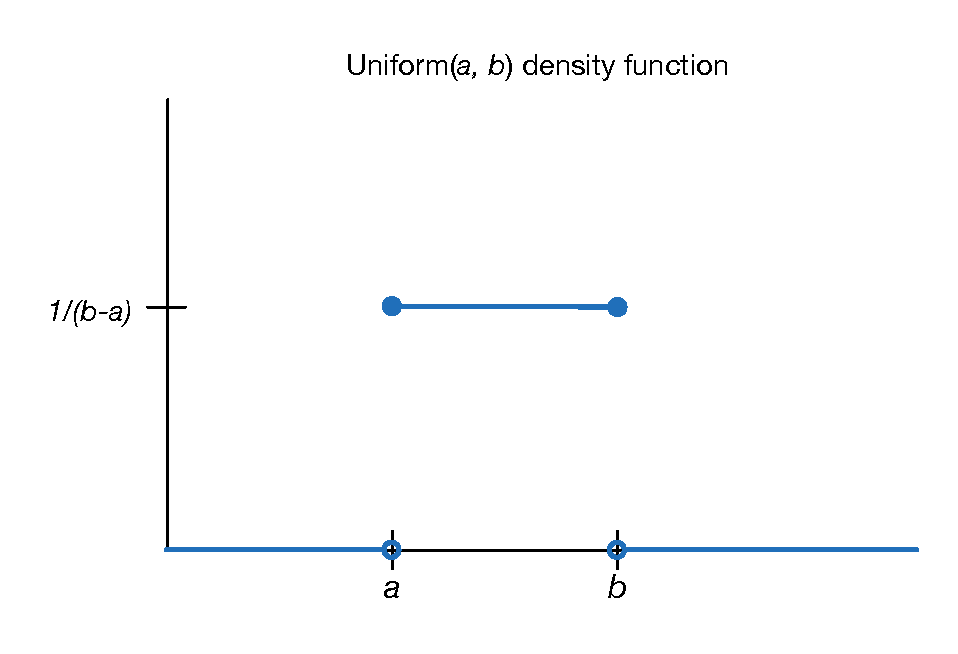
\includegraphics[width=8cm]{uniformdensity.eps}
\end{figure}
The uniform density is a horizontal line between $a$ and $b$ and is 0 otherwise. (Does this make sense?) What is the height of the horizontal line? Since the integral of a probability density must integrate to 1, and since the uniform density is nothing more than a box, the area of the box must be 1. For that to be the case, the height of the box must be $1 / (b-a)$. This is summarized below.

\begin{framed}
\emph{Uniform random variable}\\
  \rule{\dimexpr\linewidth-2\fboxsep-2\fboxrule}{.1pt} \\
A continuous random variable $Y$ has a \emph{uniform distribution} on the interval $[a, b]$ if the pdf of $Y$
is given by:
\[
f(y) = \begin{cases}
\frac{1}{b-a} & a \leq y \leq b \\
0 & \text{otherwise}
\end{cases}
\]
$Y$ a \emph{uniform random variable}, which we can write as $Y \sim\text{Uniform}(a,b)$.
\end{framed}

Let's do an example.

\begin{example}A circle has a radius which is uniformly distributed on the interval $[0, 1]$. What is the expected value of the area of the circle?\\

Let $Y\sim\text{Uniform}(0, 1)$. Then $Y$ has density
\[
f(y) = \begin{cases}
1 & 0 \leq y \leq 1 \\
0 & \text{otherwise}
\end{cases}
\]
The area of a circle of radius $y$ is given by $g(y) = \pi y^2$. Then the expected value of the area is:
\begin{align*}
\E[g(Y)] &= \int_{-\infty}^\infty g(y) f(y) dy \\
&= \int_0^1 \pi y^2 \: 1 dy \\
&= \pi \frac{y^3}{3} \Bigr|_0^1 \\
&= \frac{\pi}{3}
\end{align*}

\end{example}

As with every other distribution, we are interested in the mean and the variance of the uniform distribution. These are given below.

\begin{framed}
\emph{Properties of the uniform distribution}\\
  \rule{\dimexpr\linewidth-2\fboxsep-2\fboxrule}{.1pt} \\
Let  $Y$ have the \emph{uniform distribution} on the interval $[a, b]$. Then
\begin{align*}
\E(Y) &= \frac{a + b}{2} \\
Var(Y) &= \frac{(b-a)^2}{12}
\end{align*}
\end{framed}
It makes sense that the mean of the uniform distribution is halfway between the endpoints. To verify this, for $Y \sim\text{Uniform}(a, b)$ with density $f(y)$ as given above:
\begin{align*}
E(Y) &= \int_{-\infty}^\infty y f(y) dy \\
&= \int_a^b y \frac{1}{b-a} dy \\
&= \frac{1}{b-a} \frac{y^2}{2} \Bigr|_a^b \\
&= \frac{b^2 - a^2}{2(b-a)} \\
&= \frac{(b+a)(b-a)}{2(b-a)} \\
&= \frac{a+b}{2}
\end{align*}
The variance can be found similarly by computing $\E(Y^2)$ and using the Magic Variance Formula.

\subsection{Normal Distribution}
The most important and most useful continuous probability distribution is the normal distribution, also known as the Gaussian distribution or the ``bell curve'' for its familiar bell-like shape. Many observations from nature are approximately normally distributed, and we will see later that in the appropriate limit, just about everything has a normal distribution. In particular, we will see that for large enough $n$, we can approximate a binomial random variable with a normal distribution; this is especially useful since computations with the normal distribution are often easier than dealing with the pesky factorials in the binomial pmf.\\

Examples of the normal distribution from the natural (or artificial) world include:
\begin{enumerate}
\item Weights of chimpanzees (and just about any other species) follow the normal distribution.
\item Errors in scientific measurment (due to imperfect instrument and imperfect scientists) are normally distributed.
\item Scores on the SAT (and other standardized tests) are normally distributed (in this case by design).
\end{enumerate}

We define a normal distribution by its density function.

\begin{framed}
\emph{Normal distribution}\\
  \rule{\dimexpr\linewidth-2\fboxsep-2\fboxrule}{.1pt} \\
A continuous random variable $Y$ has a \emph{normal distribution} with parameters $\mu$ and $\sigma$ if its density $f(y)$ is given by
\begin{align*}
f(y) = \frac{1}{\sqrt{2 \pi \sigma^2}} e^{-\frac{(y - \mu)^2}{2 \sigma^2}}
\end{align*}
$Y$ is a \emph{normal random variable}, denoted $Y \sim \text{Normal}(\mu, \sigma)$. Sometimes $\sigma^2$ is given as the parameter instead of $\sigma$.
\end{framed}

A graph of the pdf for the normal distribution with parameters $\mu = 0$ and $\sigma = 0$ is shown below.
\begin{figure}[H]
\centering
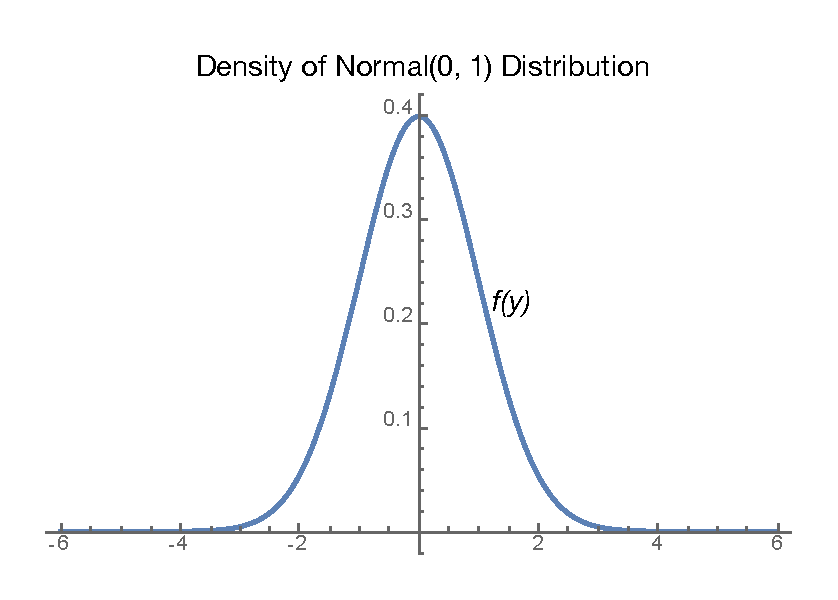
\includegraphics[width=8cm]{normalpdf2.eps}
\end{figure}

The parameters of the normal distribution, $\mu$ and $\sigma$, are the mean and standard deviation of the normal distribution.

\begin{framed}
\emph{Properties of the normal distribution}\\
  \rule{\dimexpr\linewidth-2\fboxsep-2\fboxrule}{.1pt} \\
Let $Y$ be a normal random variable with parameters $\mu$ and $\sigma$. Then
\begin{align*}
\E(Y) &= \mu \\
Var(Y) &= \sigma^2
\end{align*}
$\sigma$ is the standard deviation of $Y$.
\end{framed}

The fact that this is a valid pdf, i.e. that it integrates to 1, is a standard exercise in multivariable calculus\footnote{The usual method is to square the integral, combine the integrands into a double integral, and change from cartesian to polar coordinates.}. The normal distribution with $\mu = 0$ and $\sigma = 1$ is so prevalent that it is called the \emph{standard normal distribution}. It is repesented by the letter $Z$. 

\begin{framed}
\emph{Standard normal distribution}\\
  \rule{\dimexpr\linewidth-2\fboxsep-2\fboxrule}{.1pt} \\
The \emph{standard normal distribution} is a normal distribution with parameters $\mu = 0$ and $\sigma = 1$ and is designated by the letter $Z$. The pdf of $Z$ is:
\begin{align*}
f(z) = \frac{1}{\sqrt{2 \pi}} e^{-\frac{z^2}{2}}
\end{align*}
\end{framed}

Let $Z$ be a standard normal random variable, and suppose we wish to calculate $\P(-1 \leq Z \leq 1)$. Using the density of the standard normal:
\begin{align*}
\P(-1 \leq Z \leq 1) = \int_{-1}^1 \frac{1}{\sqrt{2 \pi}} e^{-\frac{z^2}{2}} dz
\end{align*} 
Unfortunatly, there is no nice antiderivative for the integrand, so we cannot compute the integral using the fundamental theorem of calculus. One option is to use numerical intergration techniques, which can be done using sofware packages such as Matlab or Mathematica. Another option is to use tables for the cdf of the standard normal distribition. Although this is perhaps a bit ``old-school'', it is important you know how to use these tables. There are many versions of the $Z$-table. The one I will provide (and the one which is on the course website) is the actual cdf for $Z$, i.e. is gives values for $F(z) = \P(Z \leq z)$. Since the standard normal is symmetric about 0, some tables only provide values on one side of the mean, since the others can be computed using symmetry. The table in the texbook by Wackerly et al (2008), for example, provides $\P(Z \geq z)$ for $z \geq 0$.\\

How do we compute this using a $Z$-table? Letting $F(z)$ be the cdf for the standard normal distribution, recall that for any continuous probability distribution we have:
\[
\P(a \leq Z \leq b) = F(b) - F(a)
\]
Then in this case, $\P(-1 \leq Z \leq 1) = F(1) - F(-1)$. Looking at the $Z$-table\footnote{The value of $F(z)$ is denoted by $z$ in our table. The column on the left gives us the first decimal place and tells us what row to use. Then we read across the row to match the second decimal place}, we see that $F(1) = 0.8413$ and $F(-1) = 0.1587.$ Subtracting, we obtain $\P(-1 \leq Z \leq 1) = 0.6826$.\\

Let's do an example so we can practice using a $Z$-table.

\begin{example}Let $Z$ be a standard normal random variable, and let $F(z)$ be its cdf.
\begin{enumerate}
\item Find $\P(Z > 2)$.\\

Since $\P(Z > 2) = 1 - \P(Z \leq 2) = F(2)$, we just need to find $F(2)$. Looking this up in the $Z$-table, we see that $F(2) = 0.9772$, thus $\P(Z > 2) = 1 - 0.9772 = 0.0228$.

\item Find $\P(-2 \leq Z \leq 2)$\\

$\P(-2 \leq Z \leq 2) = F(2) - F(-2)$. From the $Z$-table, $F(2) = 0.9772$ and $F(-2) = 0.0228$. Thus we have $\P(-2 \leq Z \leq 2) = 0.9772 - 0.0228 = 0.9544$.

\item Find $\P(0 \leq Z \leq 1.73)$.

$\P(0 \leq Z \leq 1.73) = F(1.73) - F(0)$. From the $Z$-table, $F(1.73) = 0.9582$ (go to the row labeled 1.7, then across to the column corresponding to 0.03). We could use the table for $F(0)$, but since the distribution is symmetric about 0, we know $F(0) = 0.5$. Subtracting, we get $\P(0 \leq Z \leq 1.73) = 0.9582 - 0.5 = 0.4582$.

\end{enumerate}
\end{example}

Before we go on, let us comment on two of the probabilities we alreadly calculated. Recall the the standard deviation of the standard normal random variable is 1. Then $\P(-1 \leq Z \leq 1)$ is the probabiltiy of falling within one standard deviation of the mean and $\P(-2 \leq Z \leq 2)$ is the probability of falling within to standard deviations of the mean. These are useful numbers to remember, since they are good guidelines for interpreting the normal distribution.

\begin{framed}
\emph{Guidelines for normal probabilities}\\
  \rule{\dimexpr\linewidth-2\fboxsep-2\fboxrule}{.1pt} \\
Let $Y$ be a random variable with a normal distribution. Then:
\begin{enumerate}
\item The probability of falling within 1 standard deviation of the mean is about 0.68
\item The probability of falling within 2 standard deviations of the mean is about 0.95
\item The probability of falling within 3 standard deviations of the mean is about 0.997
\end{enumerate}
This is known as the \emph{68-95-99.7 rule}
\end{framed}

What do we do when we don't have a normal random varible. We can transform \emph{any} random variable $Y \sim\text{Normal}(\mu, \sigma)$ into a standard normal random varible $Z$ using the following formula:
\[
Z = \frac{Y - \mu}{\sigma}
\]
In other words, we subtract the mean and divide by the standard deviation.

\begin{example}A machine produces ball bearings which diameters which are normally distributed with mean 3.0005 cm and standard deviation 0.0010 cm. Specifications require ball bearing diameters which lie in the interval $3.0000 \pm 0.0020$ cm. What fraction of the total production meets those specifications.\\

Let $Y$ be the diameter of a ball bearing produced by the machine. Then $Y \sim\text{Normal}(3.0005, 0.0010)$. We want the proability that $Y$ is within the required range, i.e. $\P(2.9980 \leq Y \leq 3.0020)$. To do this, we convert this to an interval involving the standard normal random variable $Z$. 
\begin{align*}
y &= 2.9980 & z = \frac{2.9980 - 3.0005}{0.0010} = -2.5\\
y &= 3.0020 & z = \frac{3.0020 - 3.0005}{0.0010} = 1.5
\end{align*}
So $\P(2.9980 \leq Y \leq 3.0020)$ = $\P(-2.5 \leq Z \leq 1.5)$. Looking at the $Z$-table, we find that $F(-2.5) = 0.0062$ and $F(1.5) = 0.9332$. Thus:
\[
\P(2.9980 \leq Y \leq 3.0020) = \P(-2.5 \leq Z \leq 1.5) = F(1.5) - F(-2.5) = 0.9332 - 0.0062 = 0.9270
\]
So approximately 92.7\% of the ball bearings meet the required specifications.
\end{example}

\subsection{Exponential Distribution}
The final continuous distribution we will discuss is the exponential distribution. The exponential distribution belongs to the family of gamma distributions, and is perhaps the most useful member of that family; it is the only gamma distribution we will consider in this class.\\

The exponential distribution is used to model the length of time between events which occur independently and at a constant average rate. For example, it could be used the model the length of time between customer arrivals at a restaurant or phone calls at a call center. If this reminds you of a Poisson distribution, that is good! If we have a sequence of events which occur independently from each other and at a constant average rate, then:
\begin{enumerate}
\item The Poisson distribution is a discrete distribution which measures the number of events which occur in a fixed span of time.
\item The exponential distribution is a continuous distribution which measures the amount of time between two subsequent events.
\end{enumerate}
Thus, the Poisson distribution and the exponential distribution ask different questions about the same problem.\\

The exponential distribution is also used to model the lifetime of electronic and mechanical components. Recall that we used the geometric distribution in a similar way; we did an example where the number of hours until a computer crashed was modeled as a geometric random variable. If we want to model the lifetime as a continuous random variable instead of a discrete one, then we use the exponential distribution. The exponential distribution has another similarity to the geometric distribution; as we shall see, it is also memoryless. In fact, the geometric and exponential distributions are the only two probability distributions with this property.\\

Let's define the exponential distribution, then use it to model some problems.

\begin{framed}
\emph{Exponential distribution}\\
  \rule{\dimexpr\linewidth-2\fboxsep-2\fboxrule}{.1pt} \\
A continuous random variable $Y$ has an exponential distribution with parameter $\lambda > 0$ if its density function is:
\[
f(y) = \begin{cases}
\lambda e^{-\lambda y} & y \geq 0 \\
0 & y < 0
\end{cases}
\]
$Y$ is an exponential random variable with parameter $\lambda$, which is denoted $Y \sim \text{Exponential}(\lambda)$.
\end{framed}

You will sometimes see the exponential density written as $(1/\beta)e^{-y/\beta}$. I prefer the above version, since the parameter $\lambda$ is the same as that in the Poisson distribution, i.e. the average rate at which the events occur.\\

As always, we first verify that the exponential distribution is a valid probability density.

\begin{align*}
\int_{-\infty}^\infty f(y) dy &= \int_0^\infty \lambda e^{-\lambda y} dy \\
&= \lambda \lim_{t \rightarrow \infty} \int_0^t e^{-\lambda y} dy \\
&= \lambda \left( -\frac{1}{\lambda} \right) \lim_{t \rightarrow \infty} e^{-\lambda y}\Bigr|_0^t \\
&= -\left( \lim_{t\rightarrow\infty} e^{-\lambda t} - 1 \right) \\
&= 1
\end{align*}
since the limit of the exponential in the second-to-last line above is 0.\\

Next, we find the expected value and variance of the exponential distribution.

\begin{framed}
\emph{Properties of the exponential distribution}\\
  \rule{\dimexpr\linewidth-2\fboxsep-2\fboxrule}{.1pt} \\
Let $Y$ be an exponential random variable with parameter $\lambda > 0$. Then
\begin{align*}
\E(Y) &= \frac{1}{\lambda}\\
Var(Y) &= \frac{1}{\lambda^2}
\end{align*}
\end{framed}
For the expected value, if $Y \sim \text{Exponential}(\lambda)$ has density $f(y)$, then
\begin{align*}
\E(Y) &= \int_{-\infty}^{\infty} y f(y) dy \\
&= \int_0^{\infty} \lambda y e^{-\lambda y} dy \\
&= \lambda \lim_{t\rightarrow \infty} \int_0^t \lambda y e^{-\lambda y} \\
&= \lambda \lim_{t\rightarrow \infty} \left( -\frac{1}{\lambda}y e^{-\lambda y}\Bigr|_0^t + \frac{1}{\lambda}\int_0^t e^{-\lambda y}dy \right) & \text{integration by parts} \\
&= -\lim_{t\rightarrow \infty} t e^{-\lambda t} + 0 + \frac{1}{\lambda} \int_0^\infty e^{-\lambda y} dy \\
&= \frac{1}{\lambda}
\end{align*}
where in the second-to-last line the limit is 0 (exponentials grow faster than any power) and the integral is 1 (since it's the integral of the exponential density). Similarly, using the Magic Variance Formula and integrating by parts twice, we can prove the variance of an exponential random variable.

\begin{example}While procrastinating studying for APMA 1650, you decide to create a website for your cat. Suppose your cat's website gets an average of 5 unique visits per hour. What is the probability that your cat will go more than 30 minutes without a visitor?\\

We can model the number of visits to your cat's website per hour as a Poisson distribution with parameter $\lambda = 5$ and the time between visits as an exponential distribution with the same parameter $\lambda = 5$. In this case, we are interested in the time between visits. Let $X \sim \text{Exponential}(5)$. Then $X$ has density $f(x) = 5 e^{-5x}$
Then since we are working in units of hours, the probability we want is $\P(X \geq 1/2)$.
\begin{align*}
\P(X \geq 1/2) &= \int_{1/2}^{\infty} 5 e^{-5x} dx \\
&= -\frac{5}{5} e^{-5x}\Bigr|_{1/2}^\infty \\
&= e^{-5/2} \approx 0.082
\end{align*}
\end{example}

Just as the geometric distribution is memoryless, the exponential distribution is memoryless. If we think of this in terms of the lifetime of, say, a light bulb, this means that the probability of the bulb burning out in the next 30 minutes is the same whether we just turned the light bulb on or whether it has been on for 5 days. To prove the memoryless property of the exponential distibution, it will be useful to have an expression for the cdf of the exponential distribution.

\begin{framed}
\emph{Cumulative distribution function (cdf) for the exponential distribution}\\
  \rule{\dimexpr\linewidth-2\fboxsep-2\fboxrule}{.1pt} \\
Let $Y$ be an exponential random variable with parameter $\lambda > 0$. Then its cdf $F(y)$ is given by:
\begin{align*}
F(y) = \begin{cases}
1 - e^{\lambda y} & y > 0 \\
0 & y \leq 0
\end{cases}
\end{align*}
\end{framed}
To see this, we just integrate the density function. Let $Y \sim\text{Exponential}(\lambda)$, and let $f(y)$ be its density. For $Y \leq 0$, the cdf $F(y) = 0$. (Why is this the case?) For $y > 0$, we use the definition of the cdf to get:
\begin{align*}
F(y) &= \P(Y \leq y) \\
&= \int_{-\infty}^y f(t) dt \\
&= \int_{0, y} \lambda e^{-\lambda t} dt \\
&= -e^{-\lambda t}\Bigr|_0^y \\
&= 1 - e^{-\lambda y}
\end{align*}

We can use this to show the memoryless property of the exponential distribution.

\begin{framed}
\emph{Memoryless property of the exponential distribution}\\
  \rule{\dimexpr\linewidth-2\fboxsep-2\fboxrule}{.1pt} \\
Let $Y$ be a geometric random variable with parameter $\lambda$. Then for all $a$ and $b$
\begin{align*}
\P(Y > a + b | Y > a) = \P(Y > b)
\end{align*}
\end{framed}
To see this, we first use the exponential cdf $F(y)$ to see that
\[
\P(Y > y) = 1 - \P(Y \leq y) = 1 - F(y) = 1 - (1 - e^{-\lambda y}) = e^{-\lambda y}
\]
Using this and the definition of conditional probability:
\begin{align*}
\P(Y > a + b | Y > a) &= \frac{ \P(Y > a + b \cap Y > a) }{ \P(Y > a )} \\
&= \frac{ \P(Y > a + b ) }{ \P(Y > a )} \\
&= \frac{e^{-\lambda(a+b)}}{e^{-\lambda a}} \\
&= e^{-\lambda b} \\
&= \P(Y > b)
\end{align*}

We can also use the cdf of the exponential distibution to find the median. To do this we solve $F(m) = 1/2$, where $F(y)$ is the exponential cdf.
\begin{align*}
F(m) &= \frac{1}{2} \\
1 - e^{-\lambda m} &= \frac{1}{2} \\
e^{-\lambda m} &= \frac{1}{2} \\
- \lambda m &= \log\left( \frac{1}{2} \right) = -\log 2 \\
m &= \frac{\log 2}{\lambda}
\end{align*} 
The median of the exponential distribution is thus a little smaller than the mean (by a factor of $\log 2 \approx 0.693)$.

\subsection{Bounds on Probabilities}
Sometimes what we are interested in is the probability of an outlier event, i.e. the probability that a random variable deviates from the mean by more than a certain amount. Of course, if we know the exact probability distribution, this is not hard to calculate. However, even if we don't know the probability distribution, we can still obtain upper bounds on the probability of outlier events. In this section we will look at two inequalities which allow us to do exactly this. Markov's Inequality can be used if only the mean is known, but it gives us the weakest bound. Chebyshev's Inequality is a better bound, but required knowledge of both the mean and the variance. The moral of the story is: the more information we have about a probability distribution, the better estimates we can get.

\subsubsection{Markov's Inequality}
We first look at Markov's Inequality, which gives the probability that a nonnegative random variable exceeds a certain threshold in terms of the expected value of the random variable. To use Markov's Inequality, we only need to know the expected value.

\begin{framed}
\emph{Markov's Inequality}\\
  \rule{\dimexpr\linewidth-2\fboxsep-2\fboxrule}{.1pt} \\
Let $Y$ be a nonnegative random variable with expected value $E(Y)$. If $a > 0$, then
\begin{align*}
\P(Y \geq a) \leq \frac{\E(Y)}{a}
\end{align*}
\end{framed} 
To see that this is true, let $I_a$ be the indicator random variable for the event $(Y \geq a)$, i.e. define $I_a$
 by
 \[
I_a = \begin{cases}
1 & Y \geq a \\
0 & \text{otherwise, i.e. if }Y < a
\end{cases}
\]
Next note that $a I_a \leq Y$. To see this is true, if $Y < a$, then $a I_a = 0 \leq Y$ since $Y$ is nonnegative (this is why we require $Y$ to be nonnegative). If $Y \geq a$, then $a I_a = a \leq Y$. Thus we have:
\begin{align*}
\E(a I_a) &\leq E(Y) \\
a\left[ 1 \cdot \P(Y \geq a) + 0 \cdot \P(Y < a) \right] &\leq E(Y) \\
a \P(Y \geq a) &\leq E(Y) \\
\P(Y \geq a) &\leq E(Y)
\end{align*}
where in the second line we used the definition of the expected value of a discrete random variable.

\begin{example}Suppose we randomly select an article from a journal where the mean article length is known to be 1000 words. Find an upper bound on the probability that an article exceeds 1400 words in length.\\

Let $Y$ be the length of an article in this journal. We know nothing about $Y$ except that its mean is 1000. Certainly $Y$ is nonnegative, thus we can find an upper bound for $\P(Y \geq 1400)$ using Markov's inequality:
\[
\P(Y \geq 1400) \leq \frac{E(y)}{1400} = \frac{1000}{1400} \approx 0.71
\]
This is not a great upper bound, but it's better than nothing!
\end{example}


\subsubsection{Chebyshev's Inequality}
The second inequality we will look at is Chebyshev's Inequality, which gives the probability that a random variable deviates from its mean by more than a certain amount. This does not require a nonnegative random variable, but it does require knowledge of both the mean and the variance of a random variable.

\begin{framed}
\emph{Chebyshev's Inequality}\\
  \rule{\dimexpr\linewidth-2\fboxsep-2\fboxrule}{.1pt} \\
Let $Y$ be a nonnegative random variable with expected value $\E(Y)$ and variance $Var(Y)$. If $a > 0$, then
\begin{align*}
\P(\abs{Y - E(Y)}\geq a) \leq \frac{Var(Y)}{a^2}
\end{align*}
\end{framed} 
Note the absolute value sign inside the probability for Chebyshev's Inequality. This means that Chebyshev's Inequality gives a bound for the probability of deviating from the mean \emph{in either direction}. Contrast this to Markov's Inequality, which is a bound on the probaility of \emph{exceeding} a certain value.\\

To see this is true, take the nonnegative random variable $(Y - \E(Y))^2$ and substitute it into Markov's Inequality along with the constant $a^2$. This gives us:
\[
\P([Y - \E(Y)]^2 \geq a^2) \leq \frac{E[(Y - E(Y)]^2}{a^2} = \frac{Var(Y)}{a^2}
\]
where the last equality uses the definition of variance. Then since $\abs{x} \geq a$ if and only if $x^2 \geq a^2$,
\[
\P(\abs{X - \E(X)} \geq a) = \P([X - \E(X)]^2 \geq a^2) \leq \frac{Var(Y)}{a^2}
\]
which is Chebyshev's Inequality.\\

Sometimes we like to measure deviation from the mean in terms of ``numbers of standard deviations''. For the normal distribution, this is encapsulated in the 68-95-99.7 rule. We can state Chebyshev's Inequality in these terms if we like. Let $Y$ be a random variable with mean $\mu$ and variance $\sigma^2$. Recall that the standard deviation is the square root of the variance, so the standard deviation of $Y$ is $\sigma$. Then Chebyshev's Inequality states that the probability of deviating at least $k$ standard deviations from the mean is bounded by:
\[
\P(\abs{Y - \mu}\geq k \sigma) \leq \frac{1}{k^2}
\]
To see this is true, just take $a = k \sigma$ in Chebyshev's Inequality above.

\begin{example}Suppose we randomly select an article from a journal article length is distributed with a mean 1000 words and a standard deviation of 150 words. Find an upper bound on the probability that an article is outside of the range 600 - 1400 words?\\

Let $Y$ be the length of an article in this journal. Here we know both the mean and the standard deviation of $Y$, we can can use Chebyshev's Inequality. We are looking for the probability that $Y$ deviates from the mean by at least 400. Recalling that the variance is the square of the standard deviation:
\[
\P(Y \geq 1400 \cup Y \leq 600) = \P(\abs{Y - 1000} \geq 400 ) \leq \frac{Var(Y)}{400^2} = \frac{150^2}{400^2} \approx 0.14
\]
Let's compare this to the bound we got in the previous example using Markov's Inequality. Since $(Y \geq 1400) \subset (Y \geq 1400 \cup Y \leq 600)$, using the properties of probability:
\[\
\P(Y \geq 1400) \leq \P(Y \geq 1400 \cup Y \leq 600) \leq 0.14
\]
This is a much better bound than we got from Markov's Inequality. If we have reason to suspect that the distribution of $Y$ is symmetric about the mean, we can divide $\P(Y \geq 1400 \cup Y \leq 600)$ by 2 to get:
\[
\P(Y \geq 1400) \leq \frac{\P(Y \geq 1400 \cup Y \leq 600)}{2} \leq \frac{0.14}{2} = 0.07
\]
\end{example}
which is even better! It is important that we can only do this is we have (or suspect we have) a symmetric probability distribution. This is not true in general.\\

Just for comparison purposes, let's see how much better this bound is if we know the exact distribution of $Y$. Suppose $Y$ is normally distributed with the same parameters, i.e. $Y \sim \text{Normal}(1000, 150)$. Then, standardizing to the standard normal random variable $Z$ with cdf $F(y)$:
\begin{align*}
\P(600 \leq Y \leq 1400) &= \P \left( \frac{600 - 1000}{150} \leq Z \leq \frac{1400 - 1000}{150} \right) \\
&= \P( -2.67 \leq Z \leq 2.67) \\
&= F(2.67) - F(-2.67) \\
&= 0.9962 - 0.0038 = 0.9924
\end{align*}
Thus we have:
\[
\P(Y \geq 1400 \cup Y \leq 600) = 1 - \P(600 \leq Y \leq 1400) \leq 0.0076
\]
Although Chebyshev's Inequality gives a decent bound on the probability of outliers, there is no substitute for knowing the actual probability distribution!
\end{document}

